\chapter{Precision estimation tests}
The automated assembly system has a number of properties in terms of precision:
\begin{enumerate}
\item Motion stage movement repeatability.
\item Image acquiring repeatability.
\item Precision of pattern recognition.
\item Possible movements of the sensors while picking them up and down with the vacuum pick up tool.
\item \ldots
\end{enumerate}
In order to investigate this properties a series of tests were done.
\\Real sensors will be very thin (around 200~um). This fact makes them very fragile. Even though dummy sensors, which will be used for further experiments, is a bit thicker (around 300~um), they are still too fragile for the first tests, because the bottom surface of the pick up tool and the plane underneath testing samples are not yet parallel enough. That is why for the first pick up and down tests we used glass samples. They have the same dimentions and represent close enough the properties of silicon sensors. Moreover, they are much cheaper, so that in case of test failure (sample breakes) it will not be such a big problem as if silicon sample crashes. Despite all mentioned above, none of glass samples where crashed.
\\Even though we did not do the pick up test with silicon samples, there is still an opportunity to get some information of the pick up and down precision of the silicon samples without \underline{direct testing of them [?]}. By making a full range of tests with glass samples, we will be able to say how pick up and down influences the precision. Based on this results we will be able to approximately predict the precision of pick up and down tests with silicon samples. Later, when parallelness of the bottom surface of the pick up tool and samples will be provided, we will be able to confirm the results of the prediction. More information concerning precision of pick up and down of silicon samples one can see in the section XX.

\section{Pattern recognition precision tests}

For investigation of the pattern recognition precision the folowing tests were done. During these tests samples were not moved, so that the additional errors by vacuum pick up and down can be excluded.   \ldots
\subsection{Pattern recognition on the painted corner of a glass dummy}
In the very first test we investigated the pattern recognition on the corner of the sample. Thin pieces of glass with a silver painted corner (Figure \ref{fig:painted_corner}) were used for the tests as an approximation of a silicon sensor.

\begin{figure}[ht]\centering
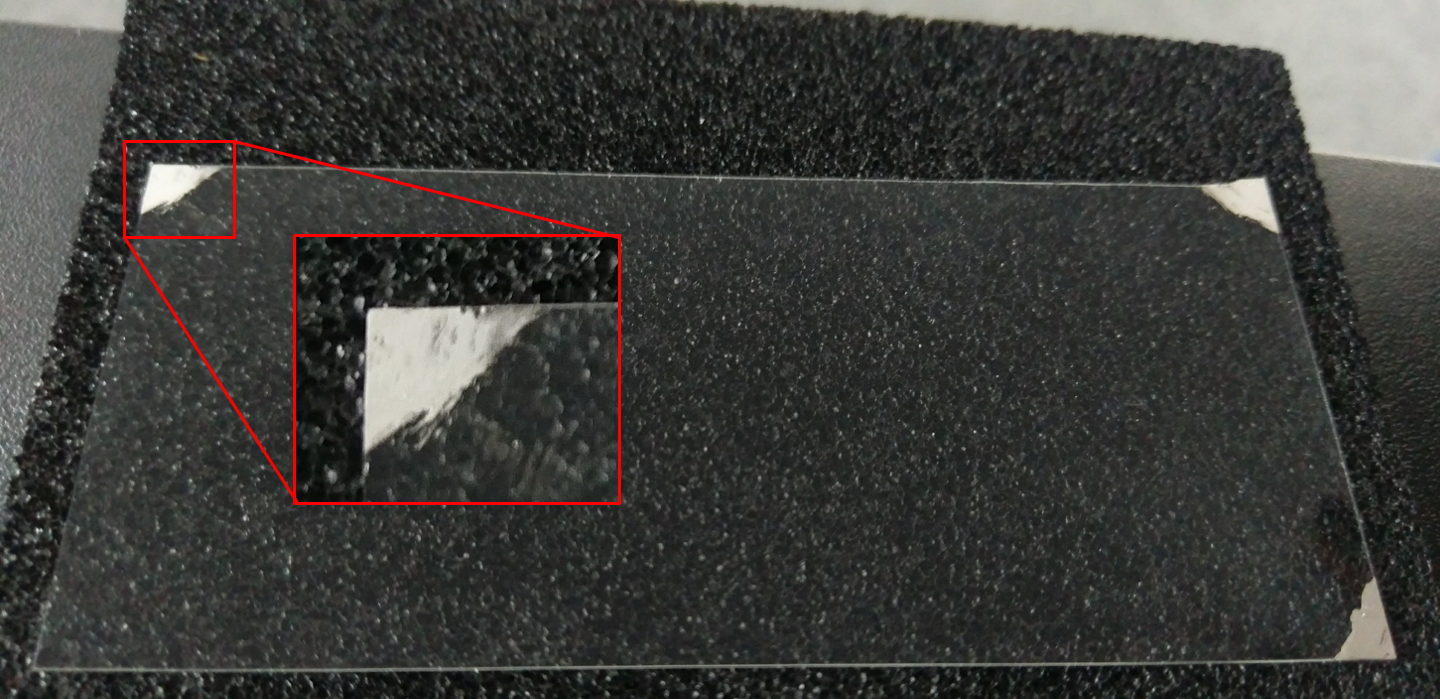
\includegraphics[width=0.8\linewidth]{Data/Precision_tests/Painted_corner.png}
\caption{Glass sample with silver painted corner.}
\label{fig:painted_corner}
\end{figure}

The step-by-step outline of this test is listed below:
\begin{enumerate}
\item Move to the image acquiring position.
\item Acquire Image and run pattern recognition.
\item Move aside for 5~mm \underline{in all axes (?)}.
\item Move to the image acquiring position.
\item Acquire Image and run pattern recognition.
\item Save data of the current iteration and go to the next one.
\end{enumerate}

After each step software saves the difference between measured cordinates before and after moving the arm with the camera. The distributions of these values are showed in Figure \ref{fig:corner_x}, Figure \ref{fig:corner_y} and Figure \ref{fig:corner_theta}. The test had 100~iterations done in a row.

\begin{figure}[ht]\centering
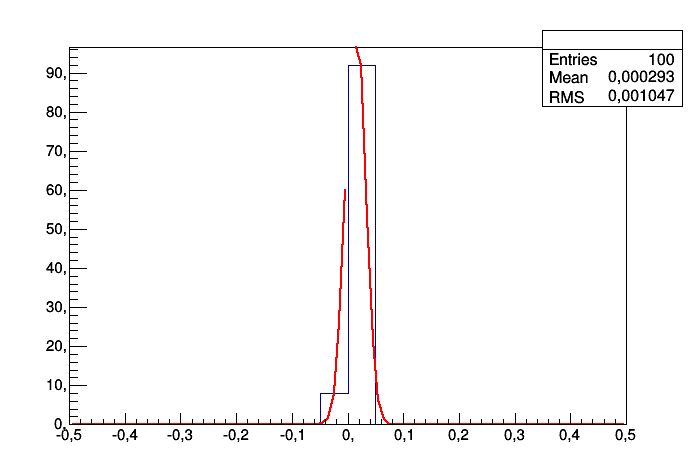
\includegraphics[width=0.8\linewidth]{Data/Precision_tests/Corner_c_x.png}
\caption{Distribution of the differnece between detected X coordinate of the master image before and after moving the arm in each iteration.}
\label{fig:corner_x}
\end{figure}

\begin{figure}[ht]\centering
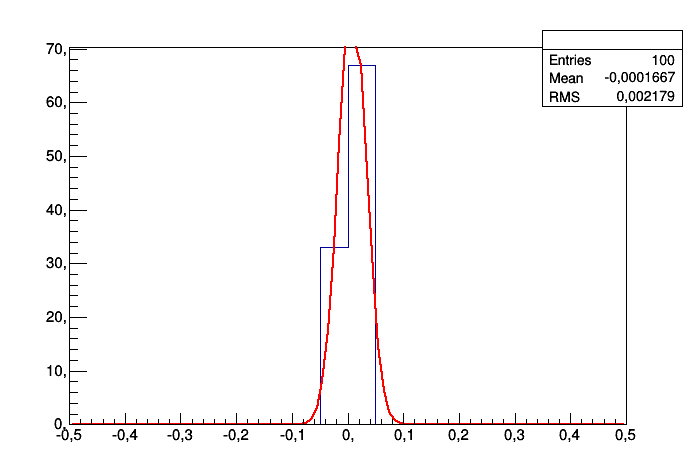
\includegraphics[width=0.8\linewidth]{Data/Precision_tests/Corner_c_y.png}
\caption{Distribution of the differnece between detected Y coordinate of the master image before and after moving the arm in each iteration.}
\label{fig:corner_y}
\end{figure}

\begin{figure}[ht]\centering
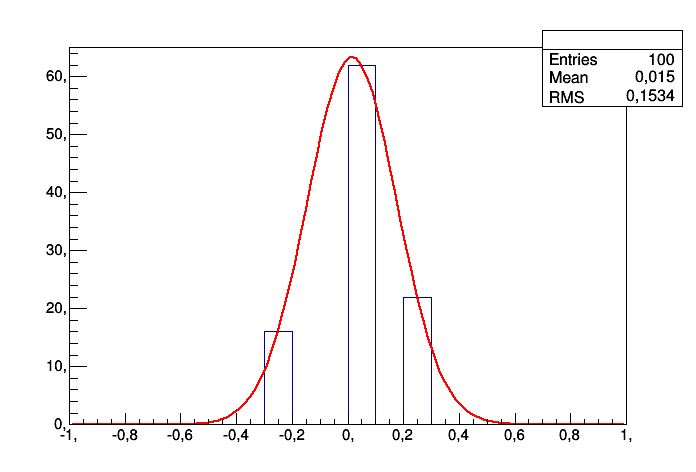
\includegraphics[width=0.8\linewidth]{Data/Precision_tests/Corner_c_theta.png}
\caption{Distribution of the differnece between detected angle orientation of the master image relaticely to the acquired image before and after moving the arm in each iteration.}
\label{fig:corner_theta}
\end{figure}

Looking at the Figures \ref{fig:corner_x} and \ref{fig:corner_y} one can see that the X, Y detection of the pattern recognition is enough precise for the project (\underline{1-2~um of error [?]}), while the theta detection results do not look so precise. There are several reasons of such behavior. The main one them is shown on the Figure \ref{fig:corner_threshold}.
\\Silver painted surface is not flat in 100~um scale. Due to this roughness different amount of light reflects to the camera. That is why the painted corner contains various shades of grey, \underline{which [?]} in some points are darker, than the table underneath the sample (background). All these result into the picture one can see in the Figure \ref{fig:corner_threshold}. This kind of pictures has random distribution of dark areas on it. That is why the pattern recognition algorithm has such error while comparing two pictures (master template and acquired image) with random distribution of black areas. Moreover, this kind of tests lasts around one hour, which is long enough for the sun light to change its luminosity. Even though all reasonably possible measures were done to prevent such effect, the acuired image is very sensetive for light. For example, during a sunny day the threshold varies for 20 units (the color depth is 256) even with closed jalousie. \underline{[should I mention it...?]}

\begin{figure}[ht]\centering
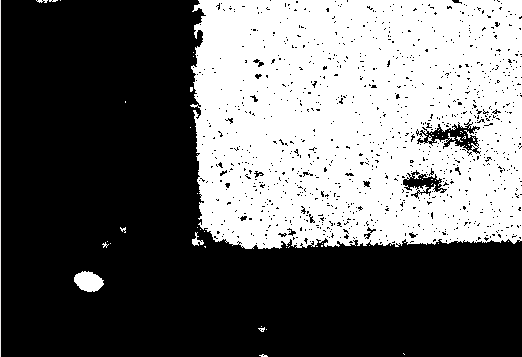
\includegraphics[width=0.8\linewidth]{Data/Precision_tests/Corner_thresholded.png}
\caption{The view of the corner after applying the Threshold.}
\label{fig:corner_threshold}
\end{figure}

\subsection{Pattern recognition on the marker of the dummy sensor}

The same test, but with dummy silicon sensor and real marker on it, was done. Before the test marker was aligned as much close to zero degrees as possible. At the Figure \ref{fig:thresholded_marker} one can see that the edge of the marker after applying Threshold is almost perfect (+/- one pixel). This fact itself is already a proof that Threashold step of pattern recognition is feasible.

\begin{figure}[ht]\centering
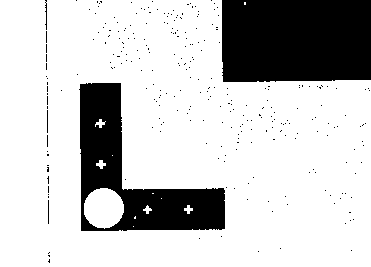
\includegraphics[width=0.8\linewidth]{Data/Precision_tests/Thresholded_marker.png}
\caption{Sensor marker after applying Threshold.}
\label{fig:thresholded_marker}
\end{figure}

The Distribution of X and Y coordinates are shown on the Figure XX
The results of the test is shown on the Figure ...





A screenshot of the application during the test is shown on the Figure \ref{fig:marker_pattern_recognition_screenshot}. On the pattern recognition curve one can see that exactly at 0 degree there is a underline{fluctuation (a short upward shot) (?)}. 

\begin{figure}[ht]\centering
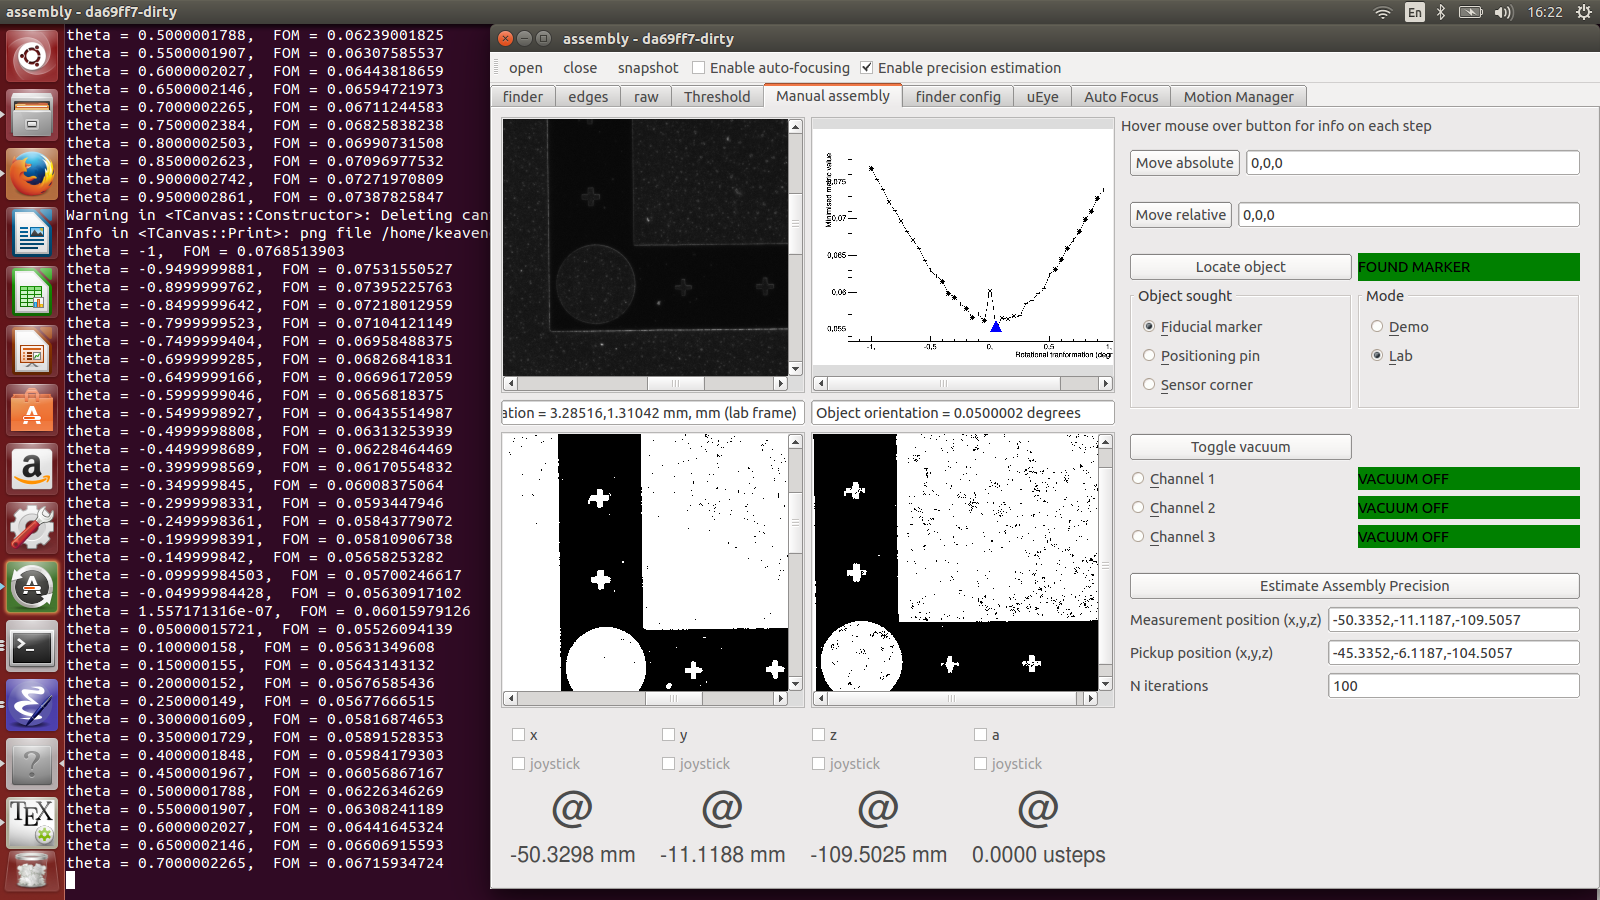
\includegraphics[width=0.8\linewidth]{Data/Precision_tests/Marker_pattern_recognition_screenshot.png}
\caption{Screenshot of application during precision extimation test with dummy silicon sensor and marker on it.}
\label{fig:marker_pattern_recognition_screenshot}
\end{figure}

\section{Arm and camera movements repeatability }

1) Make a photo
2) Move aside
3) Move back
4) Make control photo

\section{Vaccuum pick-up and -down precision}

0) Move to measurement position
1) Corner position
2) Move to pre-pickup position (!)
3) Move to pickup
4) Toggle vacuum 
5) Move up
6) Move down
7) Release vacuum
8) Move to pre-pick-up
9) Move to measurement position
10) Corner position

